% Options for packages loaded elsewhere
\PassOptionsToPackage{unicode}{hyperref}
\PassOptionsToPackage{hyphens}{url}
\PassOptionsToPackage{dvipsnames,svgnames,x11names}{xcolor}
%
\documentclass[
  beamerpaper,
  DIV=11,
  numbers=noendperiod,
  aspectratio=54]{scrreprt}

\usepackage{amsmath,amssymb}
\usepackage{iftex}
\ifPDFTeX
  \usepackage[T1]{fontenc}
  \usepackage[utf8]{inputenc}
  \usepackage{textcomp} % provide euro and other symbols
\else % if luatex or xetex
  \usepackage{unicode-math}
  \defaultfontfeatures{Scale=MatchLowercase}
  \defaultfontfeatures[\rmfamily]{Ligatures=TeX,Scale=1}
\fi
\usepackage{lmodern}
\ifPDFTeX\else  
    % xetex/luatex font selection
  \setmonofont[Scale=0.6]{Source Code Pro}
\fi
% Use upquote if available, for straight quotes in verbatim environments
\IfFileExists{upquote.sty}{\usepackage{upquote}}{}
\IfFileExists{microtype.sty}{% use microtype if available
  \usepackage[]{microtype}
  \UseMicrotypeSet[protrusion]{basicmath} % disable protrusion for tt fonts
}{}
\makeatletter
\@ifundefined{KOMAClassName}{% if non-KOMA class
  \IfFileExists{parskip.sty}{%
    \usepackage{parskip}
  }{% else
    \setlength{\parindent}{0pt}
    \setlength{\parskip}{6pt plus 2pt minus 1pt}}
}{% if KOMA class
  \KOMAoptions{parskip=half}}
\makeatother
\usepackage{xcolor}
\usepackage[left=.7in,right=.7in,marginparsep=.25in]{geometry}
\setlength{\emergencystretch}{3em} % prevent overfull lines
\setcounter{secnumdepth}{-\maxdimen} % remove section numbering
% Make \paragraph and \subparagraph free-standing
\ifx\paragraph\undefined\else
  \let\oldparagraph\paragraph
  \renewcommand{\paragraph}[1]{\oldparagraph{#1}\mbox{}}
\fi
\ifx\subparagraph\undefined\else
  \let\oldsubparagraph\subparagraph
  \renewcommand{\subparagraph}[1]{\oldsubparagraph{#1}\mbox{}}
\fi


\providecommand{\tightlist}{%
  \setlength{\itemsep}{0pt}\setlength{\parskip}{0pt}}\usepackage{longtable,booktabs,array}
\usepackage{calc} % for calculating minipage widths
% Correct order of tables after \paragraph or \subparagraph
\usepackage{etoolbox}
\makeatletter
\patchcmd\longtable{\par}{\if@noskipsec\mbox{}\fi\par}{}{}
\makeatother
% Allow footnotes in longtable head/foot
\IfFileExists{footnotehyper.sty}{\usepackage{footnotehyper}}{\usepackage{footnote}}
\makesavenoteenv{longtable}
\usepackage{graphicx}
\makeatletter
\def\maxwidth{\ifdim\Gin@nat@width>\linewidth\linewidth\else\Gin@nat@width\fi}
\def\maxheight{\ifdim\Gin@nat@height>\textheight\textheight\else\Gin@nat@height\fi}
\makeatother
% Scale images if necessary, so that they will not overflow the page
% margins by default, and it is still possible to overwrite the defaults
% using explicit options in \includegraphics[width, height, ...]{}
\setkeys{Gin}{width=\maxwidth,height=\maxheight,keepaspectratio}
% Set default figure placement to htbp
\makeatletter
\def\fps@figure{htbp}
\makeatother

\usepackage{titling}
\usepackage{fancyhdr, blindtext}
\usepackage{xcolor}
\usepackage{soul}
\usepackage{pagecolor}
\usepackage{booktabs}
\usepackage{longtable}
\usepackage{array}
\usepackage{multirow}
\usepackage{wrapfig}
\usepackage{float}
\usepackage{colortbl}
\usepackage{pdflscape}
\usepackage{tabu}
\usepackage{threeparttable}
\usepackage{threeparttablex}
\usepackage[normalem]{ulem}
\usepackage{makecell}
\usepackage{tcolorbox}
\usepackage[]{Oswald}
\usepackage{lipsum}

\definecolor{merkgreen}{RGB}{202,211,68}
\definecolor{merkdarkgreen}{RGB}{52,93,70}
\definecolor{merkyellow}{RGB}{247,233,9}

\definecolor{bggray}{rgb}{0.95,0.95,0.95}
\pagestyle{fancy}
\pretitle{\begin{center}
  
\includegraphics[width=5in,height=3.5in]{../img/logo_Merkanzia.pdf}\LARGE\\}
  \pagecolor{merkdarkgreen}
\posttitle{\end{center}}
\fancyhf{}
\newpage
\newpagecolor{merkgreen}
% \begin{tcolorbox}[
%     title="Prezzi",
% %   opacityback=1,  % this does not work
% %   colback=white,  % this is not what I want
% ]
\fancyfoot[R]{\footnotesize \textit{www.merkanzia.com info@merkanzia.com}}
\fancyfoot[L]{\footnotesize \textit{Merkanzia GmbH, La Toscana in Svizzera}}
\usepackage{booktabs}
\usepackage{longtable}
\usepackage{array}
\usepackage{multirow}
\usepackage{wrapfig}
\usepackage{float}
\usepackage{colortbl}
\usepackage{pdflscape}
\usepackage{tabu}
\usepackage{threeparttable}
\usepackage{threeparttablex}
\usepackage[normalem]{ulem}
\usepackage{makecell}
\usepackage{xcolor}
\KOMAoption{captions}{tableheading}
\makeatletter
\makeatother
\makeatletter
\makeatother
\makeatletter
\@ifpackageloaded{caption}{}{\usepackage{caption}}
\AtBeginDocument{%
\ifdefined\contentsname
  \renewcommand*\contentsname{Table of contents}
\else
  \newcommand\contentsname{Table of contents}
\fi
\ifdefined\listfigurename
  \renewcommand*\listfigurename{List of Figures}
\else
  \newcommand\listfigurename{List of Figures}
\fi
\ifdefined\listtablename
  \renewcommand*\listtablename{List of Tables}
\else
  \newcommand\listtablename{List of Tables}
\fi
\ifdefined\figurename
  \renewcommand*\figurename{Figure}
\else
  \newcommand\figurename{Figure}
\fi
\ifdefined\tablename
  \renewcommand*\tablename{Table}
\else
  \newcommand\tablename{Table}
\fi
}
\@ifpackageloaded{float}{}{\usepackage{float}}
\floatstyle{ruled}
\@ifundefined{c@chapter}{\newfloat{codelisting}{h}{lop}}{\newfloat{codelisting}{h}{lop}[chapter]}
\floatname{codelisting}{Listing}
\newcommand*\listoflistings{\listof{codelisting}{List of Listings}}
\makeatother
\makeatletter
\@ifpackageloaded{caption}{}{\usepackage{caption}}
\@ifpackageloaded{subcaption}{}{\usepackage{subcaption}}
\makeatother
\makeatletter
\@ifpackageloaded{tcolorbox}{}{\usepackage[skins,breakable]{tcolorbox}}
\makeatother
\makeatletter
\@ifundefined{shadecolor}{\definecolor{shadecolor}{rgb}{.97, .97, .97}}
\makeatother
\makeatletter
\makeatother
\makeatletter
\makeatother
\ifLuaTeX
  \usepackage{selnolig}  % disable illegal ligatures
\fi
\IfFileExists{bookmark.sty}{\usepackage{bookmark}}{\usepackage{hyperref}}
\IfFileExists{xurl.sty}{\usepackage{xurl}}{} % add URL line breaks if available
\urlstyle{same} % disable monospaced font for URLs
\hypersetup{
  pdftitle={I nostri Prodotti},
  pdfauthor={Merkanzia},
  colorlinks=true,
  linkcolor={blue},
  filecolor={Maroon},
  citecolor={Blue},
  urlcolor={Blue},
  pdfcreator={LaTeX via pandoc}}

\title{I nostri Prodotti}
\usepackage{etoolbox}
\makeatletter
\providecommand{\subtitle}[1]{% add subtitle to \maketitle
  \apptocmd{\@title}{\par {\large #1 \par}}{}{}
}
\makeatother
\subtitle{Unsere Produckte aus Toskana}
\author{Merkanzia}
\date{November 23, 2023\\
\strut \\
\strut \\
info@merkanzia.com}

\begin{document}
\maketitle
\ifdefined\Shaded\renewenvironment{Shaded}{\begin{tcolorbox}[enhanced, frame hidden, interior hidden, breakable, borderline west={3pt}{0pt}{shadecolor}, sharp corners, boxrule=0pt]}{\end{tcolorbox}}\fi

\begin{table}

\caption{\label{tbl-panel-panino}Panini Porchetta /
Finocchiona}\begin{minipage}[t]{\linewidth}
\subcaption{\label{tbl-panel-panino-1}Ciabatta rustica }

\tabularnewline

\fontsize{16}{18}\selectfont
\begin{tabular}{>{\raggedright\arraybackslash}p{16cm}}
\toprule
\begingroup\fontsize{18}{20}\selectfont \textbf{Sandwich Porchetta / Finocchiona}\endgroup\\
\midrule
Ciabatta rustica mit Finocchiona oder mit Porchetta. Zutaten: Pecorino Semistagionato, Friarelli oder getrocknete Tomaten.\\
\bottomrule
\end{tabular}

\end{minipage}%
\newline
\begin{minipage}[t]{\linewidth}

\raisebox{-\height}{

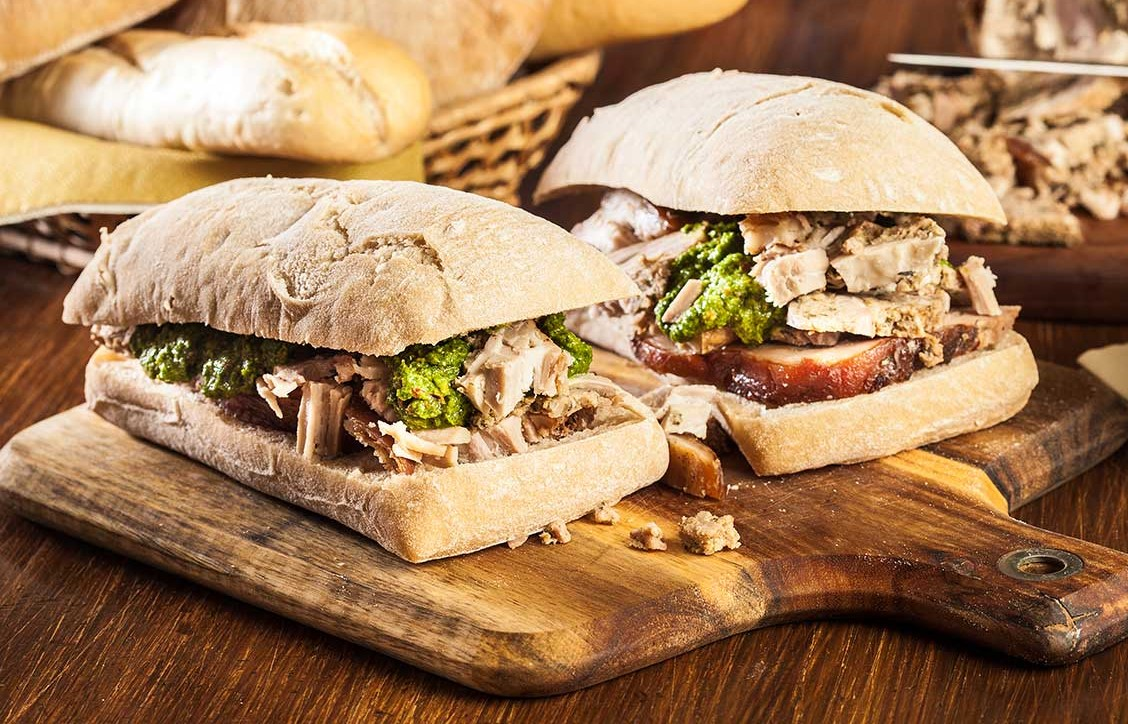
\includegraphics{../img/paninoporchetta.jpg}

}

\end{minipage}%

\end{table}

\begin{table}

\caption{\label{tbl-panel-fleisch}Finocchiona}\begin{minipage}[t]{\linewidth}
\subcaption{\label{tbl-panel-fleisch-1}Fenkelsalami }

\tabularnewline

\fontsize{16}{18}\selectfont
\begin{tabular}{>{\raggedright\arraybackslash}p{16cm}}
\toprule
\begingroup\fontsize{18}{20}\selectfont \textbf{Finocchiona}\endgroup\\
\midrule
Die typische Salami mit Fenchel aus der Toskana, angereichert mit der Anerkennung der Geschützten Geografischen Identifikation.\\
\bottomrule
\end{tabular}

\end{minipage}%
\newline
\begin{minipage}[t]{\linewidth}

\raisebox{-\height}{

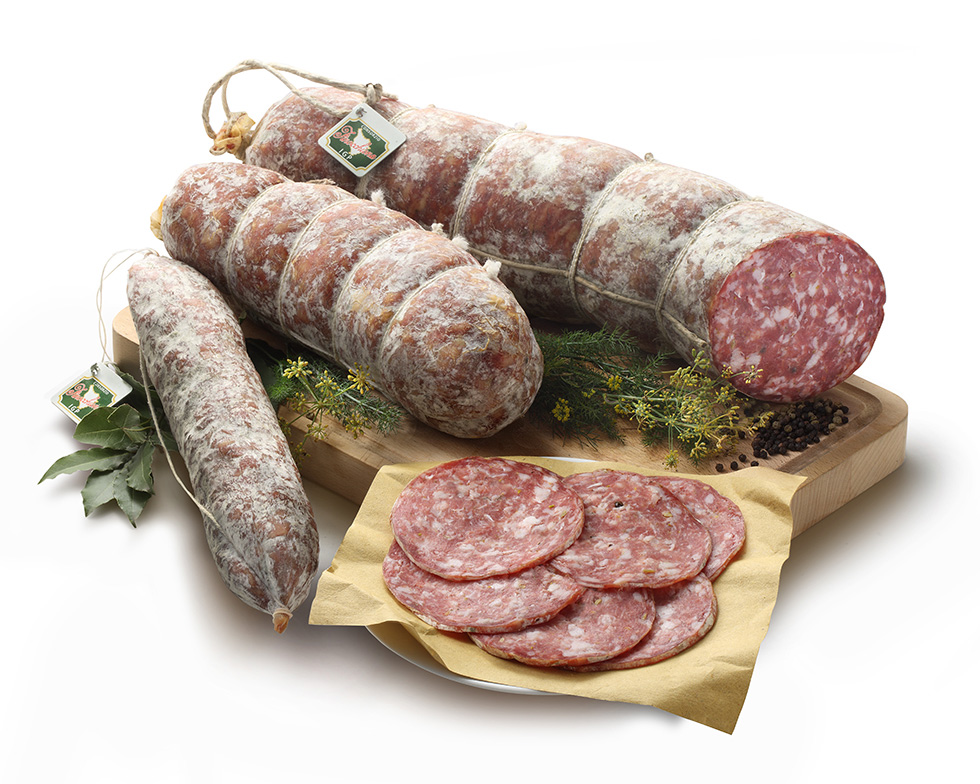
\includegraphics{../img/Finocchiona-IGP.jpg}

}

\end{minipage}%

\end{table}

\break

\begin{table}

\caption{\label{tbl-panel-fleisch2}Porchetta}\begin{minipage}[t]{\linewidth}
\subcaption{\label{tbl-panel-fleisch2-1}Schweinbraten }

\tabularnewline

\fontsize{16}{18}\selectfont
\begin{tabular}{>{\raggedright\arraybackslash}p{16cm}}
\toprule
\begingroup\fontsize{18}{20}\selectfont \textbf{Porchetta}\endgroup\\
\midrule
Schweinbraten gewürzt mit einer Mischung aus Salz, Knoblauch, Rosmarin, Pfeffer, Kräutern und wilden Fenchelblüte.\\
\cmidrule{1-1}
Im Holzbackofen gebacken.\\
\bottomrule
\end{tabular}

\end{minipage}%
\newline
\begin{minipage}[t]{\linewidth}

\raisebox{-\height}{

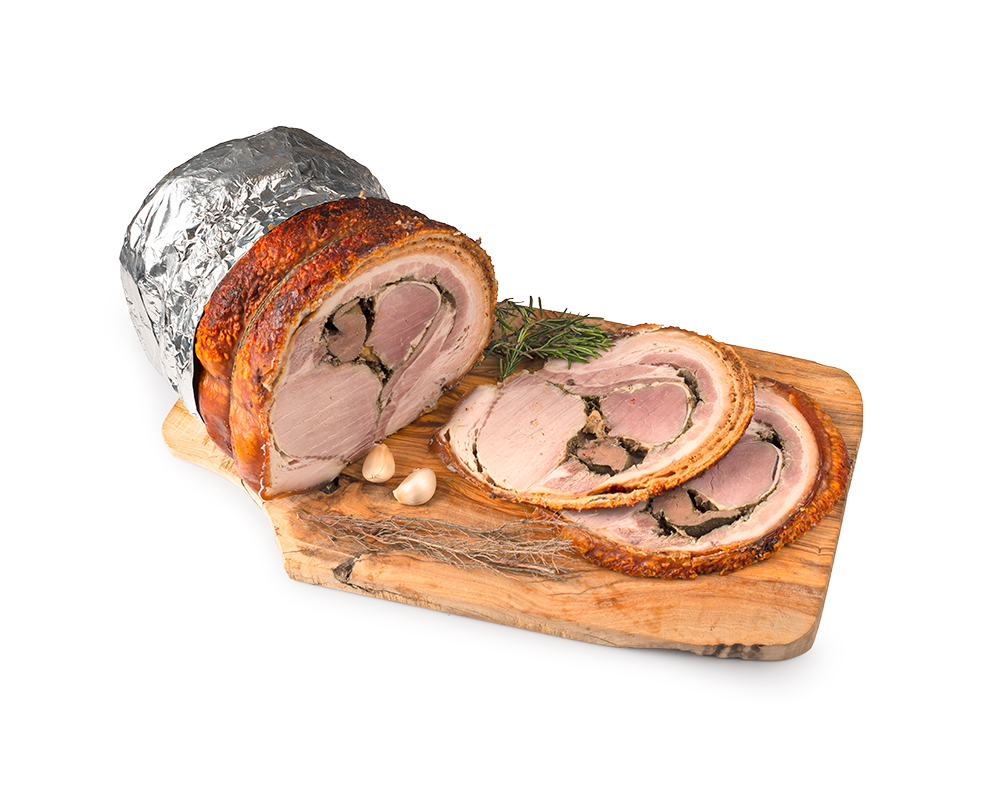
\includegraphics{../img/Porchetta-Tronchetto-cotto-a-legna.jpg}

}

\end{minipage}%

\end{table}

\begin{table}

\caption{\label{tbl-panel-cheese}Pecorino}\begin{minipage}[t]{\linewidth}
\subcaption{\label{tbl-panel-cheese-1}Sua Eccellenza il Grande }

\tabularnewline

\fontsize{16}{18}\selectfont
\begin{tabular}{>{\raggedright\arraybackslash}p{16cm}}
\toprule
\begingroup\fontsize{18}{20}\selectfont \textbf{il Grande}\endgroup\\
\midrule
Schafsmilch von ausgewählten italienischen Bauernhöfen. Reifung (90 Tage) auf Holzbrettern und/oder in kostbaren Terrakotta-Gefässen.\\
\bottomrule
\end{tabular}

\end{minipage}%
\newline
\begin{minipage}[t]{\linewidth}

\raisebox{-\height}{

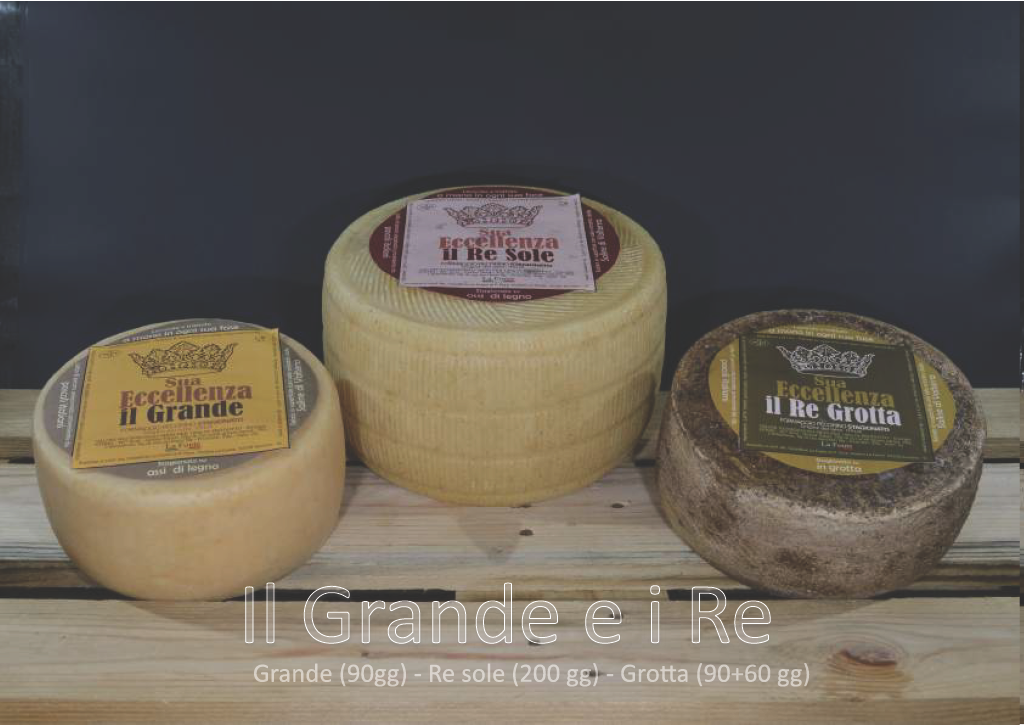
\includegraphics{../img/IlGrande1024_1.png}

}

\end{minipage}%

\end{table}

\break

\begin{table}

\caption{\label{tbl-panel-cheese2}Pecorino}\begin{minipage}[t]{\linewidth}
\subcaption{\label{tbl-panel-cheese2-1}Sua Eccellenza il Semistagionato }

\tabularnewline

\fontsize{16}{18}\selectfont
\begin{tabular}{>{\raggedright\arraybackslash}p{16cm}}
\toprule
\begingroup\fontsize{18}{20}\selectfont \textbf{il Semistagionato}\endgroup\\
\midrule
Schafsmilch von ausgewählten italienischen Bauernhöfen. Reifung (60 Tage) auf Holzbrettern und/oder in kostbaren Terrakotta-Gefässen.\\
\bottomrule
\end{tabular}

\end{minipage}%
\newline
\begin{minipage}[t]{\linewidth}

\raisebox{-\height}{

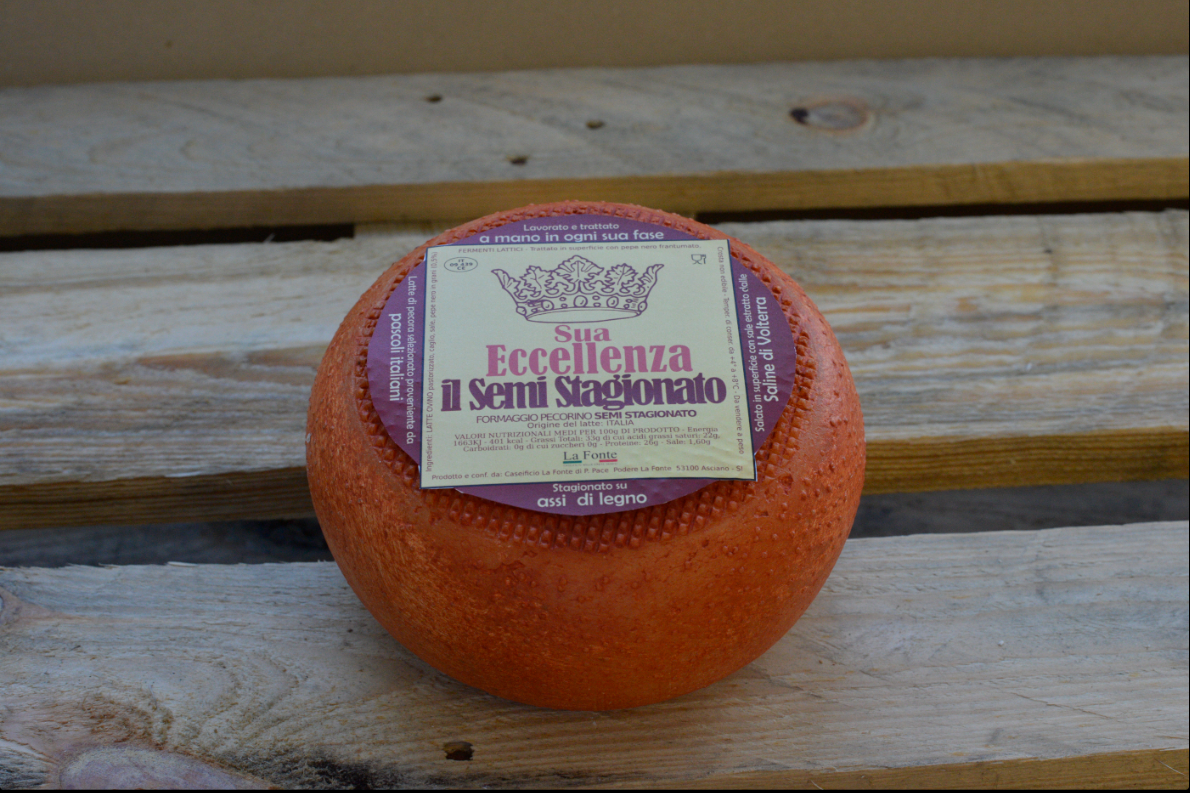
\includegraphics{../img/SuaEccellenzaIlSemiStagionato.png}

}

\end{minipage}%

\end{table}

\begin{table}

\caption{\label{tbl-panel-primi}Suppe}\begin{minipage}[t]{\linewidth}
\subcaption{\label{tbl-panel-primi-1}Ribollita aus Siena }

\tabularnewline

\fontsize{16}{18}\selectfont
\begin{tabular}{>{\raggedright\arraybackslash}p{16cm}}
\toprule
\begingroup\fontsize{18}{20}\selectfont \textbf{Ribollita}\endgroup\\
\midrule
Toskanischen Bauerntradition: Kartoffeln, Bohnen, Schwarzkohl, Wirsing, Karotten, Sellerie, Zwiebeln, Zucchini, Tomatenmark, Olivenöl, natürliche Aromen, Salz.\\
\bottomrule
\end{tabular}

\end{minipage}%
\newline
\begin{minipage}[t]{\linewidth}

\raisebox{-\height}{

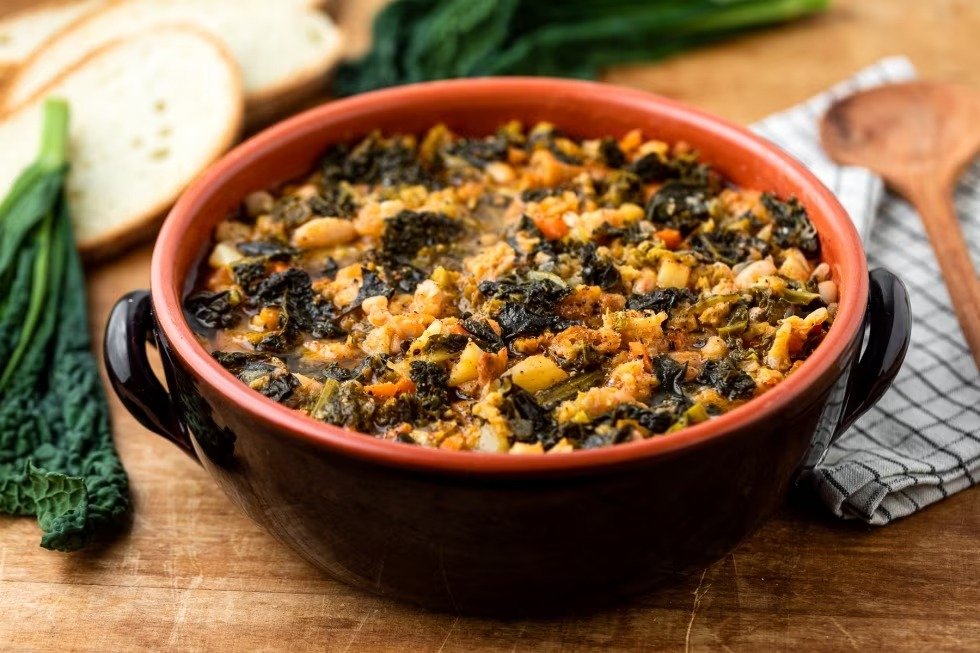
\includegraphics{../img/Ribollita.jpeg}

}

\end{minipage}%

\end{table}

\break

\begin{table}

\caption{\label{tbl-panel-primi2}Suppe}\begin{minipage}[t]{\linewidth}
\subcaption{\label{tbl-panel-primi2-1}Scottiglia aus Monte Amiata }

\tabularnewline

\fontsize{16}{18}\selectfont
\begin{tabular}{>{\raggedright\arraybackslash}p{16cm}}
\toprule
\begingroup\fontsize{18}{20}\selectfont \textbf{Scottiglia}\endgroup\\
\midrule
Ein typisches Gericht aus Pescina (Monte Amiata).\\
\cmidrule{1-1}
Rindfleisch (50\%), Schweinefleisch (39\%), Tomatenmark (10\%), Rotwein, Olivenöl, natürliche Aromen, Salz, Pfeffer.\\
\bottomrule
\end{tabular}

\end{minipage}%
\newline
\begin{minipage}[t]{\linewidth}

\raisebox{-\height}{

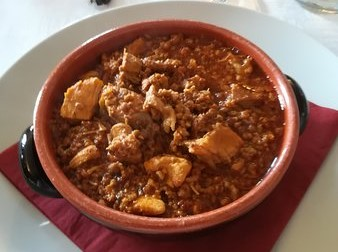
\includegraphics{../img/la-scottiglia.jpg}

}

\end{minipage}%

\end{table}

\begin{table}

\caption{\label{tbl-panel-gnocchi}Gnocchi}\begin{minipage}[t]{\linewidth}
\subcaption{\label{tbl-panel-gnocchi-1}Gnocchi Ragu }

\tabularnewline

\fontsize{16}{18}\selectfont
\begin{tabular}{>{\raggedright\arraybackslash}p{16cm}}
\toprule
\begingroup\fontsize{18}{20}\selectfont \textbf{Gnocchi al Ragu'}\endgroup\\
\midrule
Handgemachte Kartoffelgnocchi mit Fleischragout.\\
\bottomrule
\end{tabular}

\end{minipage}%
\newline
\begin{minipage}[t]{\linewidth}

\raisebox{-\height}{

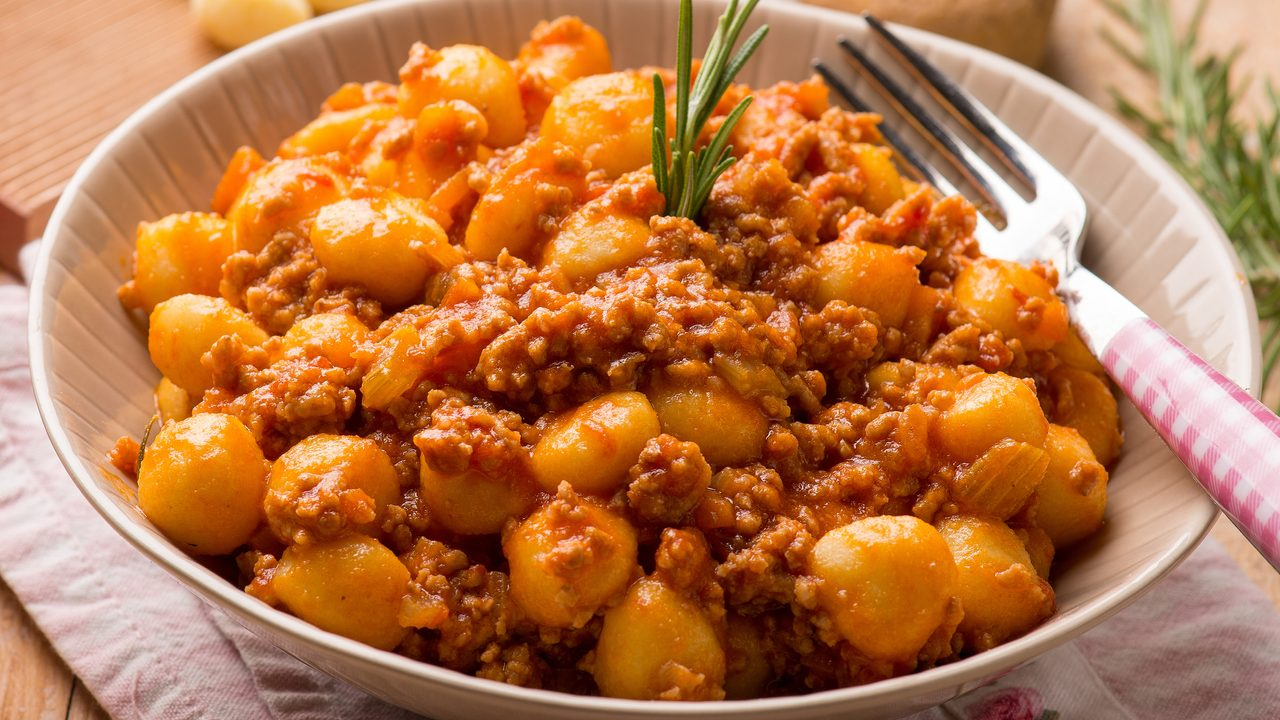
\includegraphics{../img/Gnocchi-al-Ragu-1280x720.jpg}

}

\end{minipage}%

\end{table}

\break

\begin{table}

\caption{\label{tbl-panel-aglio}Aglione Val di
Chiana}\begin{minipage}[t]{\linewidth}
\subcaption{\label{tbl-panel-aglio-1}Aglione Sosse }

\tabularnewline

\fontsize{16}{18}\selectfont
\begin{tabular}{>{\raggedright\arraybackslash}p{16cm}}
\toprule
\begingroup\fontsize{18}{20}\selectfont \textbf{Aglione}\endgroup\\
\midrule
Tomatensauce mit einer Knoblauchsorte, die in der Region Val di Chiana angebaut wird. Grössere Grösse, feineres Aroma und hohe Verdaulichkeit.\\
\bottomrule
\end{tabular}

\end{minipage}%
\newline
\begin{minipage}[t]{\linewidth}

\raisebox{-\height}{

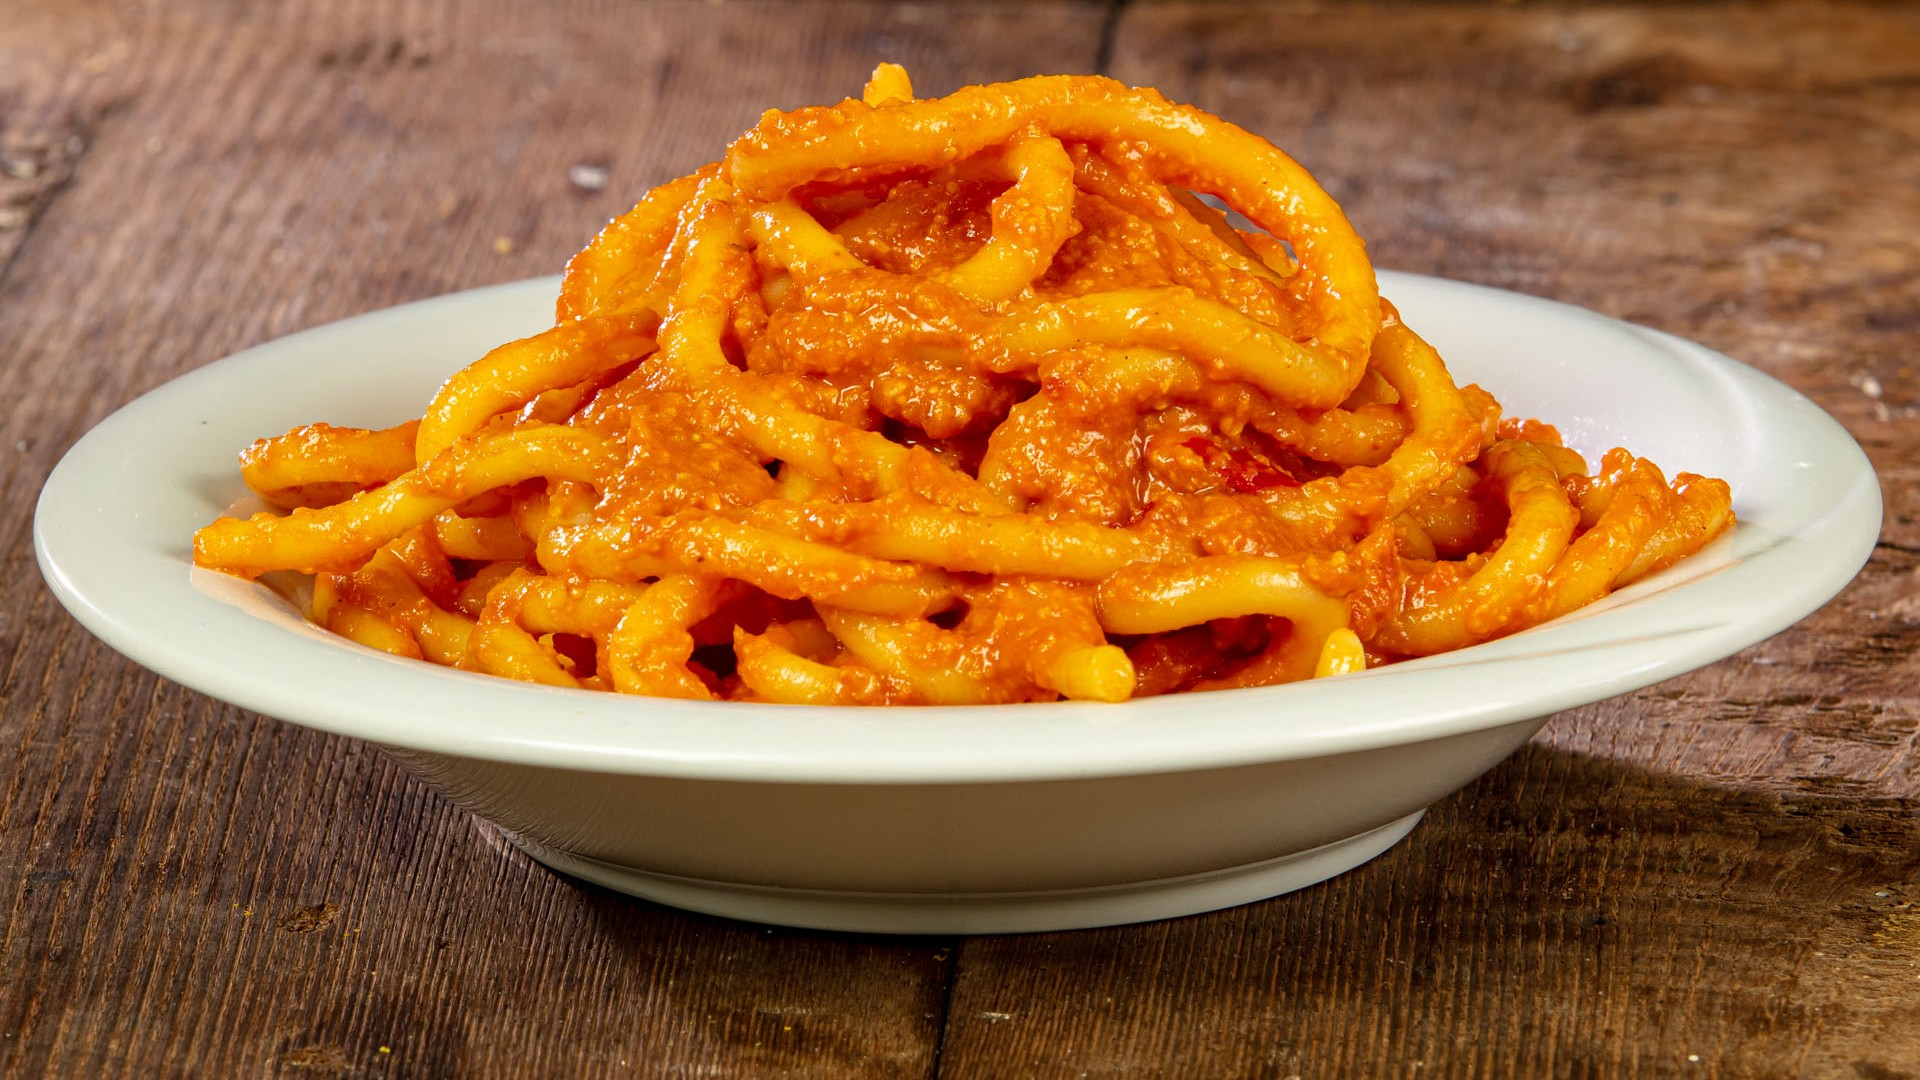
\includegraphics{../img/pici-all-aglione.jpg}

}

\end{minipage}%

\end{table}

\begin{table}

\caption{\label{tbl-panel-panza}Panzanella}\begin{minipage}[t]{\linewidth}
\subcaption{\label{tbl-panel-panza-1}Toskanischer Brotsalat }

\tabularnewline

\fontsize{16}{18}\selectfont
\begin{tabular}{>{\raggedright\arraybackslash}p{16cm}}
\toprule
\begingroup\fontsize{18}{20}\selectfont \textbf{Panzanella}\endgroup\\
\midrule
Ein armes, vegetarisches Gericht bäuerlichen Ursprungs: Trocknen Sie das Brot (um es nicht wegzuwerfen) und kombinieren Sie es mit Gemüse aus Ihrem eigenen Garten.\\
\bottomrule
\end{tabular}

\end{minipage}%
\newline
\begin{minipage}[t]{\linewidth}

\raisebox{-\height}{

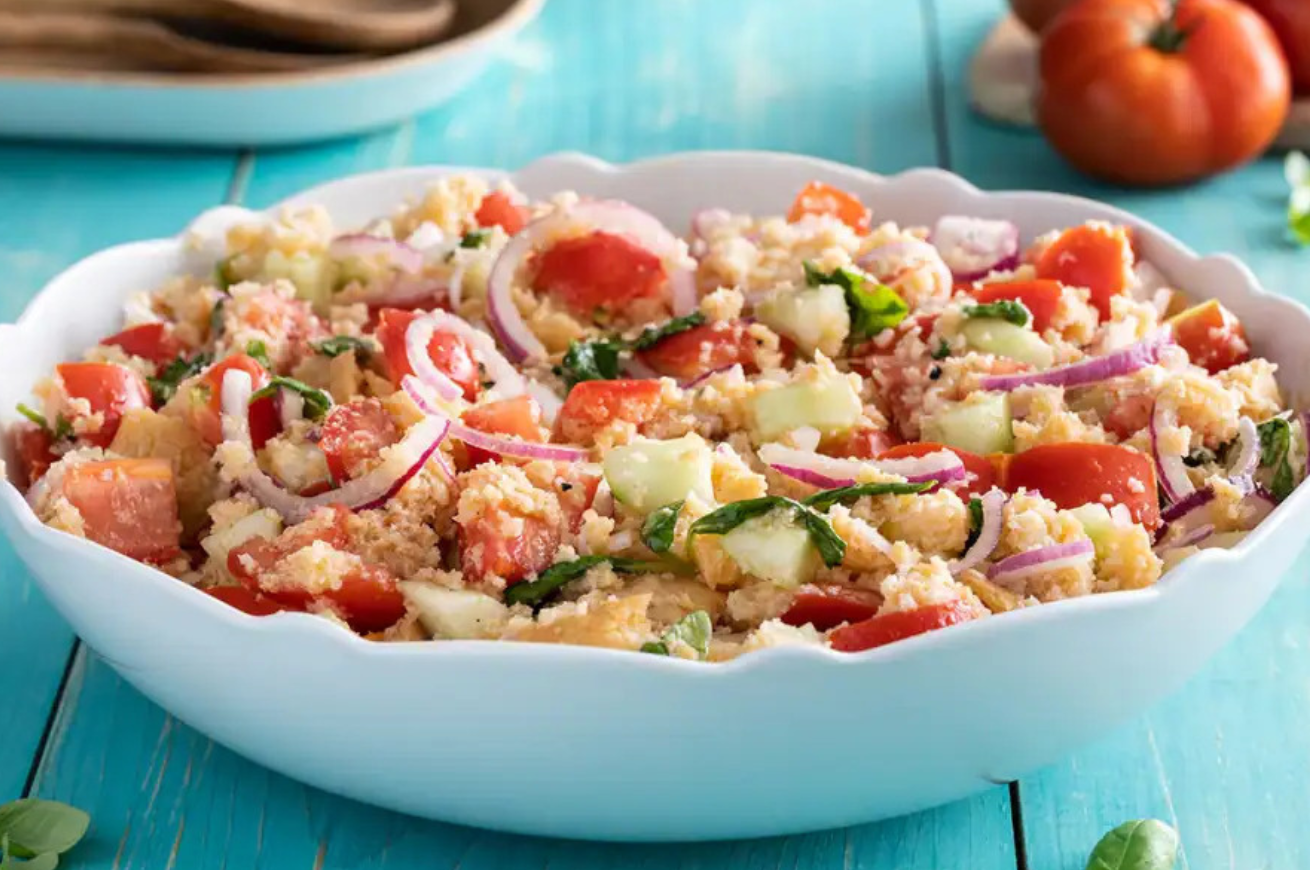
\includegraphics{../img/Panzanella.png}

}

\end{minipage}%

\end{table}

\break

\begin{table}

\caption{\label{tbl-panel-ceci}Zuppa di
Ceci}\begin{minipage}[t]{\linewidth}
\subcaption{\label{tbl-panel-ceci-1}Kichererbsen-Suppe }

\tabularnewline

\fontsize{16}{18}\selectfont
\begin{tabular}{>{\raggedright\arraybackslash}p{16cm}}
\toprule
\begingroup\fontsize{18}{20}\selectfont \textbf{Zuppa di Ceci}\endgroup\\
\midrule
Nach alter Tradition zubereitete Suppe mit frischen Produkten: hauptsächlich Kichererbsen und Schwarzkohl.\\
\bottomrule
\end{tabular}

\end{minipage}%
\newline
\begin{minipage}[t]{\linewidth}

\raisebox{-\height}{

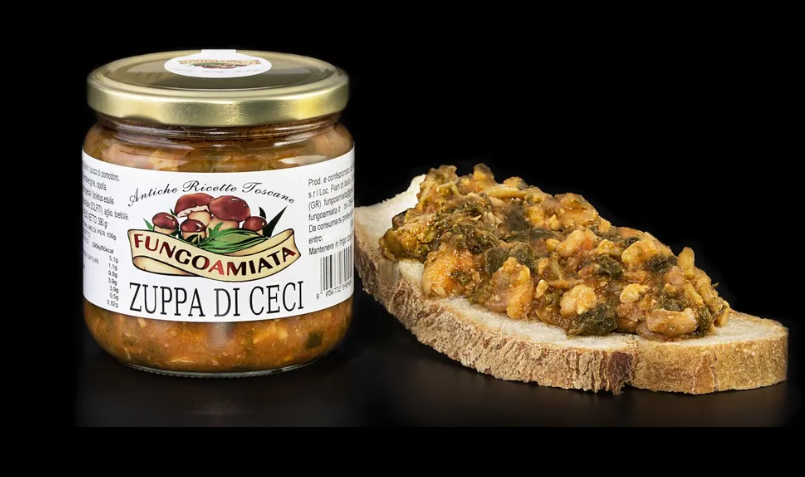
\includegraphics{../img/zuppa-ceci.png}

}

\end{minipage}%

\end{table}

\begin{table}

\caption{\label{tbl-panel-dolci}Ricciarelli alle
Mandorle}\begin{minipage}[t]{\linewidth}
\subcaption{\label{tbl-panel-dolci-1}Ricciarelli aus Siena }

\tabularnewline

\fontsize{16}{18}\selectfont
\begin{tabular}{>{\raggedright\arraybackslash}p{16cm}}
\toprule
\begingroup\fontsize{18}{20}\selectfont \textbf{Ricciarelli}\endgroup\\
\midrule
Der Ursprung der Ricciarelli geht auf das fünfzehnte Jahrhundert in Siena zurück. Es handelt sich um rautenförmige Kekse, die aus Mandelmehl hergestellt und mit Vanillezucker bestreut werden.\\
\bottomrule
\end{tabular}

\end{minipage}%
\newline
\begin{minipage}[t]{\linewidth}

\raisebox{-\height}{

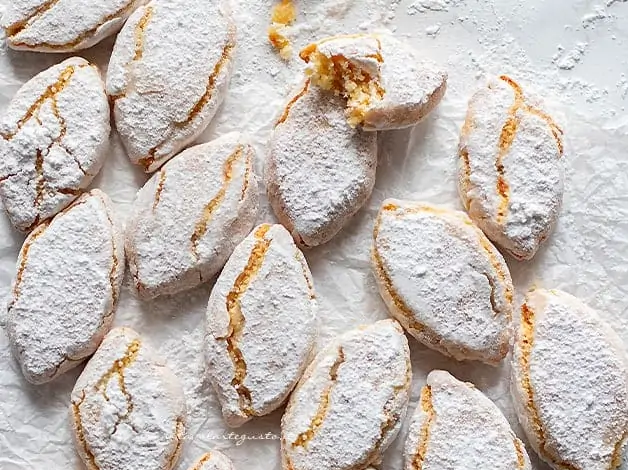
\includegraphics{../img/Ricciarelli.png}

}

\end{minipage}%

\end{table}

\begin{table}

\caption{\label{tbl-panel-cast}Castagne}\begin{minipage}[t]{\linewidth}
\subcaption{\label{tbl-panel-cast-1}Marroni aus Monte Amiata }

\tabularnewline

\fontsize{16}{18}\selectfont
\begin{tabular}{>{\raggedright\arraybackslash}p{16cm}}
\toprule
\begingroup\fontsize{18}{20}\selectfont \textbf{Marroni}\endgroup\\
\midrule
Die Marrone wächst natürlich in den Wäldern des Monte Amiata. Sie zeichnet sich durch ihre längliche Form und die Qualität ihres feinen Fruchtfleisches aus, das einen süssen und intensiven Geschmack hat.\\
\bottomrule
\end{tabular}

\end{minipage}%
\newline
\begin{minipage}[t]{\linewidth}

\raisebox{-\height}{

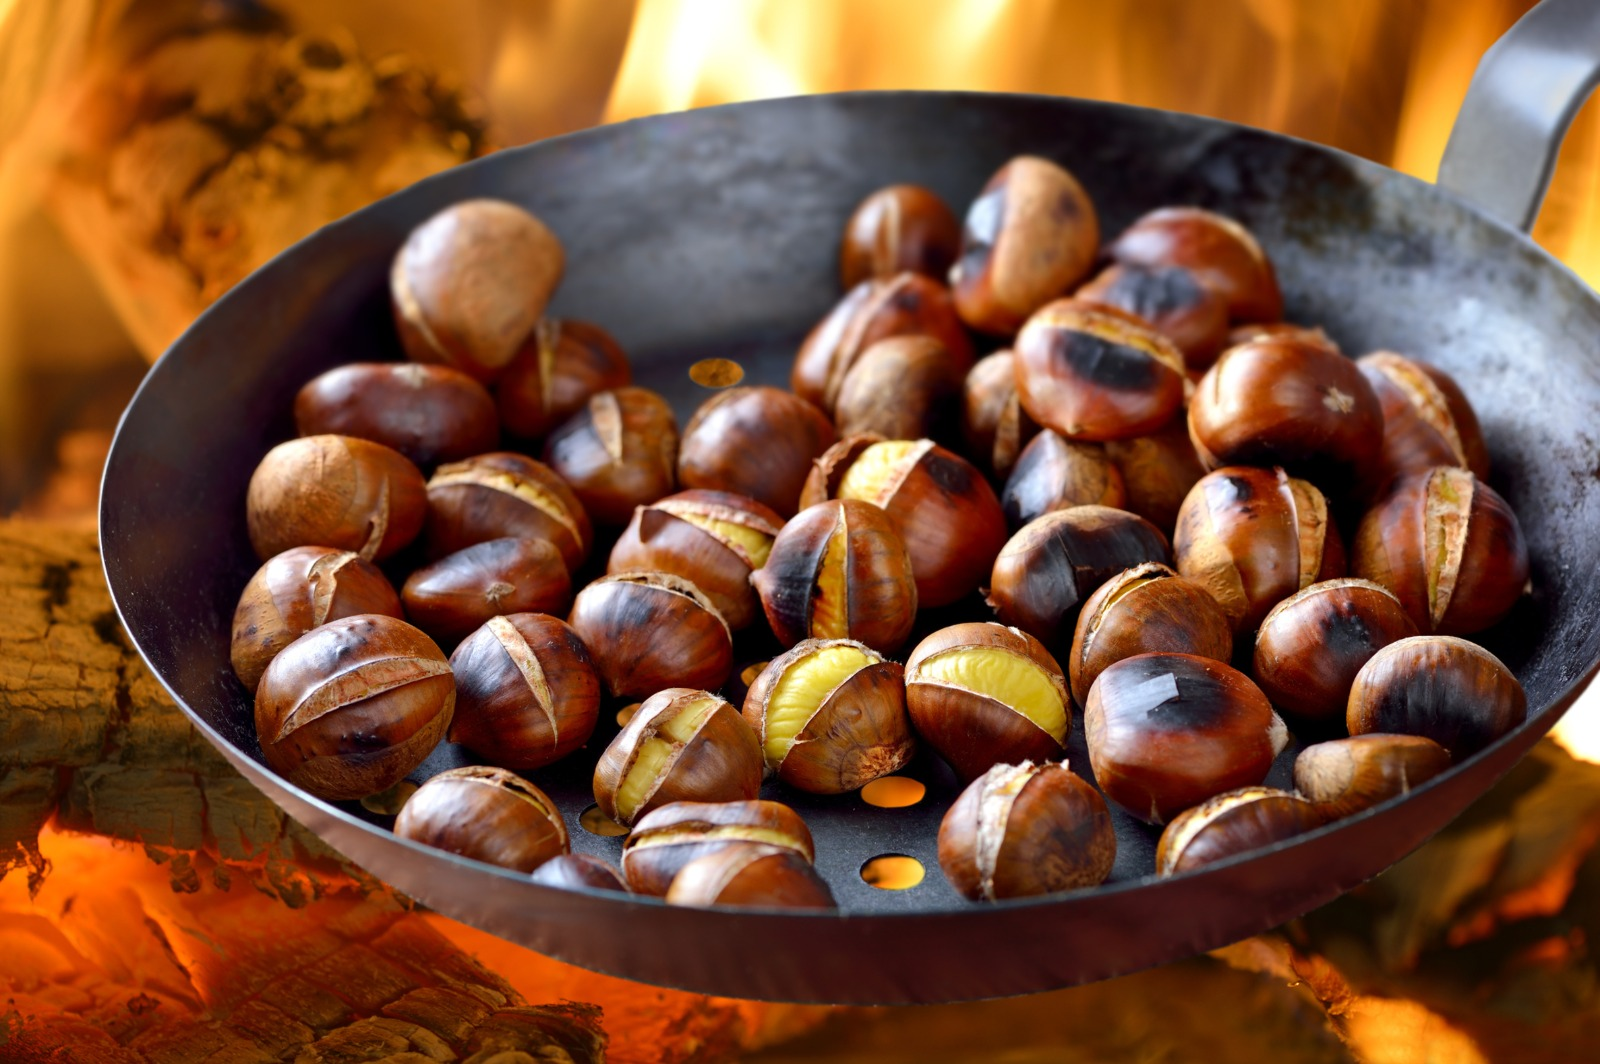
\includegraphics{../img/Marroni_padella.jpeg}

}

\end{minipage}%

\end{table}



\end{document}
